\section{Construcción del modelo}\label{sec:construccion}

Agregamos las piezas en orden, de la más sencilla a la más compleja. Cada pieza tuvo que ganarle a la mejor versión
aceptada hasta ese momento.

\subsection{Punto de partida, la media por régimen}
El modelo más simple predice para cada parcela la media de su grupo. La Fig.~\ref{fig:bases} compara varios grupos.
La media por régimen es la mejor en ambos esquemas, con 0.489\,t/ha. La media por municipio se le acerca en el
esquema A (0.510), pero en el esquema B sube a 0.955 porque, al dejar zonas fuera, muchos municipios se quedan sin
parcelas de entrenamiento. El régimen no tiene ese problema, porque se conoce para cualquier parcela. Por eso es la
base de todo lo demás.

\begin{figure}[t]
\centering
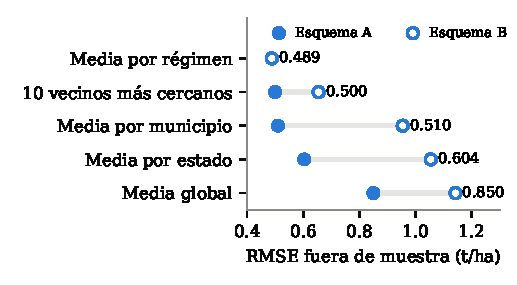
\includegraphics[width=\columnwidth]{f2_bases}
\caption{RMSE de modelos sencillos. El número es el esquema A. La media por régimen es la única que no empeora cuando
se dejan zonas completas fuera (esquema B).}
\label{fig:bases}
\end{figure}

\subsection{Rezago espacial, lo que dicen los vecinos}
Dentro de un régimen el rendimiento todavía varía, y parcelas cercanas tienden a parecerse~\cite{tobler1970}, porque
comparten suelo, clima, manejo y a veces productor. Para aprovecharlo calculamos el \emph{rezago espacial}, el
promedio del rendimiento de las parcelas de entrenamiento cercanas, ponderado por el inverso de la distancia,
\begin{equation}
\ell_i = \frac{\sum_{j\in\mathcal{N}_i} y_j / d_{ij}}{\sum_{j\in\mathcal{N}_i} 1 / d_{ij}},
\label{eq:rezago}
\end{equation}
donde $\mathcal{N}_i$ son hasta 10 vecinos del mismo régimen a menos de un radio $r$, $y_j$ su rendimiento y $d_{ij}$
la distancia en metros. Si una parcela no tiene vecinos, $\ell_i$ es la media de su régimen calculada solo con las
parcelas de entrenamiento del fold. Al calcularlo para una parcela de entrenamiento la excluimos a ella misma, tanto de
los vecinos como de esa media, para que su etiqueta no entre en su propia variable.

\textbf{El rezago de una parcela de prueba solo usa rendimientos del entrenamiento.} Lo ilustramos con un fold de la
validación que tiene 110 parcelas de entrenamiento y 28 de prueba. La parcela de prueba AGC\_073, del régimen A, tiene
tres vecinos de entrenamiento a menos de 400\,m. Están a 38, 112 y 195\,m y rindieron 4.60, 4.67 y 3.81\,t/ha. Su
rezago es 4.515, y el rendimiento declarado de la propia AGC\_073 (4.30) no interviene. La parcela AGC\_002 tiene un
único vecino a menos de 400\,m, pero ese vecino también está en el fold de prueba, así que no se usa. Sin vecinos,
AGC\_002 recibe 4.5201, la media del régimen A de las 110 parcelas de entrenamiento del fold y no la de las 138. Una
prueba automatizada comprueba esta propiedad. Altera las etiquetas de las parcelas de prueba y verifica que el rezago y
las predicciones no cambian. En la validación, 53\,\% de las parcelas de prueba no tiene vecino a 400\,m en el
entrenamiento del fold.

\textbf{Elección del radio.} El radio equilibra dos efectos (Fig.~\ref{fig:radio}). Con un radio chico casi ninguna
parcela tiene vecinos, solo el 25\,\% a 250\,m, y el rezago no aporta. Con un radio grande todas los tienen, pero el
promedio mezcla parcelas que ya no se parecen y el error sube por encima de la media por régimen. A 400\,m la mitad
de las parcelas tiene vecino y el error es el más bajo.

\begin{figure}[t]
\centering
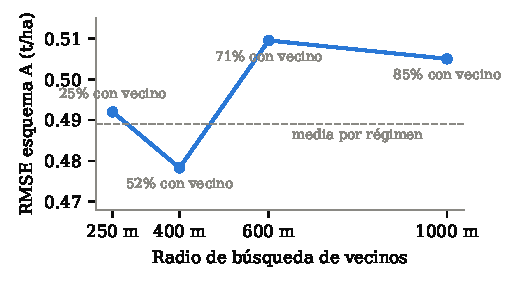
\includegraphics[width=\columnwidth]{f3_radio}
\caption{RMSE del modelo con régimen y rezago según el radio de búsqueda de vecinos. El texto indica qué fracción de
parcelas tiene al menos un vecino del mismo régimen.}
\label{fig:radio}
\end{figure}

\textbf{Otras dos decisiones.} Limitamos los vecinos al mismo régimen porque sus etiquetas se miden distinto. Como los
dos regímenes están en zonas separadas, a 400\,m el resultado es idéntico con o sin esa restricción, y la conservamos
como protección. Además, el modelo ve solo el valor del rezago y no el número de vecinos ni la distancia al más
cercano. Esas dos columnas extra agregaban ruido, y quitarlas bajó el RMSE de 0.478 a 0.470. Con ese cambio el
rezago ganó en 9 de 10 repeticiones, y fue la primera versión del rezago que lo logró.

\textbf{Prueba de permutación del rezago.} Para saber si la posición de los vecinos aporta, revolvimos las coordenadas
de las parcelas dentro de cada régimen y dejamos intactos el régimen y el rendimiento. Después recalculamos el rezago y
repetimos la validación, con 50 permutaciones y 3 repeticiones cada una. Esta prueba destruye a propósito la estructura
espacial. Si el rezago solo captara el nivel del régimen, el modelo con coordenadas revueltas predeciría igual de bien.
Ninguna de las 50 permutaciones igualó el error real, lo que da $p=0.02$, el valor más pequeño posible con 50 sorteos.
Con 200 permutaciones obtuvimos $p=0.01$ al revolver dentro del régimen y $p=0.005$ al revolver dentro del municipio.
Con 50 permutaciones dentro del municipio el resultado sigue siendo $p=0.02$. La prueba muestra que la posición de los
vecinos contiene información sobre el rendimiento además del régimen. No demuestra por sí sola que esta versión del
rezago sea mejor que otras, para eso usamos la comparación entre repeticiones.

\subsection{Variables satelitales, de clima y de topografía}\label{sec:bloques}
Sobre el modelo con régimen y rezago probamos cada bloque de variables por separado (Fig.~\ref{fig:bloques}). Ninguno
cumplió la regla. El que más se acercó fue la heterogeneidad del NDVI dentro de la parcela, que ganó en 7 de 10
repeticiones por 0.002\,t/ha, pero al revolver sus valores el modelo predijo igual ($p=0.63$). Juntar todos los
bloques satelitales empeoró el error a 0.498, porque con 138 parcelas el modelo empieza a aprender ruido. El clima
viene en celdas de unos 5\,km~\cite{funk2015,verdin2020}, así que solo distingue zonas, y eso ya lo hacen el régimen y los vecinos. También
empeoró el esquema B hasta 0.540. Por estas razones el modelo final no usa estas variables.

\begin{figure}[t]
\centering
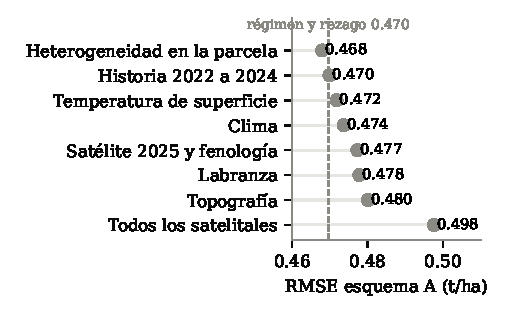
\includegraphics[width=\columnwidth]{f4_bloques}
\caption{RMSE al agregar cada bloque al modelo con régimen y rezago (línea punteada). Ninguno mejora de forma que
pase la regla de decisión.}
\label{fig:bloques}
\end{figure}

\subsection{Algoritmo}
Con las entradas fijas, régimen y rezago, comparamos algoritmos (Fig.~\ref{fig:algoritmos}). Los modelos de árboles,
bosque aleatorio y LightGBM, quedan peor que la media por régimen. Con solo tres entradas y 138 parcelas sus cortes
escalonados no tienen dónde apoyarse. Los modelos lineales, ridge, elastic net y PLS, quedan alrededor de 0.470. El
proceso gaussiano logra el menor error, 0.458, y gana al ridge en 9 de 10 repeticiones.

\begin{figure}[t]
\centering
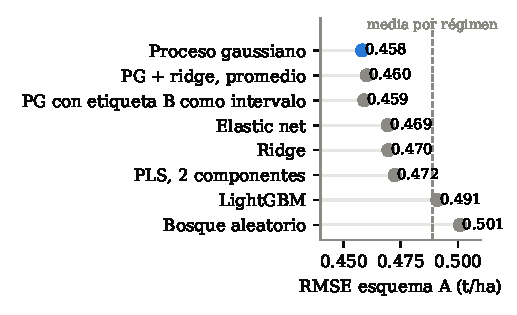
\includegraphics[width=\columnwidth]{f5_algoritmos}
\caption{RMSE de cada algoritmo con régimen y rezago. En gris, las alternativas. Las dos filas debajo del proceso
gaussiano (PG) son variantes que lo combinan con otras ideas.}
\label{fig:algoritmos}
\end{figure}

Elegimos el proceso gaussiano por tres razones además de su error. Primero, puede ajustar una relación suave y no
lineal entre el rezago y el rendimiento, mientras que un modelo lineal supone que cada t/ha de los vecinos pesa
igual en todo el rango. Segundo, tiene
pocos parámetros, tres en el kernel, que se ajustan con las propias parcelas, lo que busca limitar el sobreajuste con
muestras chicas. No lo damos por hecho y mostramos evidencia de estabilidad. El RMSE por repetición va de 0.442 a 0.503,
con desviación estándar de 0.018, y el proceso gaussiano gana a la media por régimen en 9 de 10 repeticiones. Con otras
cinco semillas de partición el promedio va de 0.452 a 0.468. Calculando el rezago sin la propia parcela, el error en el
entrenamiento de cada fold es 0.434 y el error en su fold de prueba es 0.450, una brecha de 0.016\,t/ha. Tercero, su
término de ruido absorbe parte del ruido de las etiquetas declaradas. Los procesos gaussianos ya se han usado para
predecir rendimiento con datos satelitales~\cite{you2017}.

Debemos matizar la ventaja del proceso gaussiano. Frente a un modelo lineal con las mismas entradas, la diferencia de
RMSE es de $-0.012$\,t/ha (intervalo de confianza del 95\,\% de $-0.039$ a $+0.015$, $p=0.38$), así que no lo supera de
forma significativa. Su ventaja clara es sobre los modelos de árboles.

\textbf{Ideas que no mejoraron al proceso gaussiano.} Promediarlo con un ridge (0.460) no ayudó, porque ambos usan la
misma información. Tratar la etiqueta del régimen B como un intervalo de $\pm0.25$\,t/ha para reflejar el redondeo
tampoco (0.459). Ponderar las parcelas por su área o usar una pérdida robusta de Huber mejoró menos de 0.004\,t/ha a
un ridge, sin superar al proceso gaussiano.
